% GNUPLOT: LaTeX picture with Postscript
\begingroup
  % Encoding inside the plot.  In the header of your document, this encoding
  % should to defined, e.g., by using
  % \usepackage[cp1252,<other encodings>]{inputenc}
  \inputencoding{cp1252}%
  \makeatletter
  \providecommand\color[2][]{%
    \GenericError{(gnuplot) \space\space\space\@spaces}{%
      Package color not loaded in conjunction with
      terminal option `colourtext'%
    }{See the gnuplot documentation for explanation.%
    }{Either use 'blacktext' in gnuplot or load the package
      color.sty in LaTeX.}%
    \renewcommand\color[2][]{}%
  }%
  \providecommand\includegraphics[2][]{%
    \GenericError{(gnuplot) \space\space\space\@spaces}{%
      Package graphicx or graphics not loaded%
    }{See the gnuplot documentation for explanation.%
    }{The gnuplot epslatex terminal needs graphicx.sty or graphics.sty.}%
    \renewcommand\includegraphics[2][]{}%
  }%
  \providecommand\rotatebox[2]{#2}%
  \@ifundefined{ifGPcolor}{%
    \newif\ifGPcolor
    \GPcolortrue
  }{}%
  \@ifundefined{ifGPblacktext}{%
    \newif\ifGPblacktext
    \GPblacktextfalse
  }{}%
  % define a \g@addto@macro without @ in the name:
  \let\gplgaddtomacro\g@addto@macro
  % define empty templates for all commands taking text:
  \gdef\gplbacktext{}%
  \gdef\gplfronttext{}%
  \makeatother
  \ifGPblacktext
    % no textcolor at all
    \def\colorrgb#1{}%
    \def\colorgray#1{}%
  \else
    % gray or color?
    \ifGPcolor
      \def\colorrgb#1{\color[rgb]{#1}}%
      \def\colorgray#1{\color[gray]{#1}}%
      \expandafter\def\csname LTw\endcsname{\color{white}}%
      \expandafter\def\csname LTb\endcsname{\color{black}}%
      \expandafter\def\csname LTa\endcsname{\color{black}}%
      \expandafter\def\csname LT0\endcsname{\color[rgb]{1,0,0}}%
      \expandafter\def\csname LT1\endcsname{\color[rgb]{0,1,0}}%
      \expandafter\def\csname LT2\endcsname{\color[rgb]{0,0,1}}%
      \expandafter\def\csname LT3\endcsname{\color[rgb]{1,0,1}}%
      \expandafter\def\csname LT4\endcsname{\color[rgb]{0,1,1}}%
      \expandafter\def\csname LT5\endcsname{\color[rgb]{1,1,0}}%
      \expandafter\def\csname LT6\endcsname{\color[rgb]{0,0,0}}%
      \expandafter\def\csname LT7\endcsname{\color[rgb]{1,0.3,0}}%
      \expandafter\def\csname LT8\endcsname{\color[rgb]{0.5,0.5,0.5}}%
    \else
      % gray
      \def\colorrgb#1{\color{black}}%
      \def\colorgray#1{\color[gray]{#1}}%
      \expandafter\def\csname LTw\endcsname{\color{white}}%
      \expandafter\def\csname LTb\endcsname{\color{black}}%
      \expandafter\def\csname LTa\endcsname{\color{black}}%
      \expandafter\def\csname LT0\endcsname{\color{black}}%
      \expandafter\def\csname LT1\endcsname{\color{black}}%
      \expandafter\def\csname LT2\endcsname{\color{black}}%
      \expandafter\def\csname LT3\endcsname{\color{black}}%
      \expandafter\def\csname LT4\endcsname{\color{black}}%
      \expandafter\def\csname LT5\endcsname{\color{black}}%
      \expandafter\def\csname LT6\endcsname{\color{black}}%
      \expandafter\def\csname LT7\endcsname{\color{black}}%
      \expandafter\def\csname LT8\endcsname{\color{black}}%
    \fi
  \fi
    \setlength{\unitlength}{0.0500bp}%
    \ifx\gptboxheight\undefined%
      \newlength{\gptboxheight}%
      \newlength{\gptboxwidth}%
      \newsavebox{\gptboxtext}%
    \fi%
    \setlength{\fboxrule}{0.5pt}%
    \setlength{\fboxsep}{1pt}%
    \definecolor{tbcol}{rgb}{1,1,1}%
\begin{picture}(8640.00,3772.00)%
    \gplgaddtomacro\gplbacktext{%
      \csname LTb\endcsname%%
      \put(1342,578){\makebox(0,0){\scriptsize 1e-05}}%
      \put(1342,1298){\makebox(0,0){\scriptsize 0.0001}}%
      \put(1342,2018){\makebox(0,0){\scriptsize 0.001}}%
      \put(1342,2737){\makebox(0,0){\scriptsize 0.01}}%
      \put(1342,3457){\makebox(0,0){\scriptsize 0.1}}%
      \put(2145,446){\makebox(0,0){\scriptsize 5}}%
      \put(2818,446){\makebox(0,0){\scriptsize 10}}%
      \put(3492,446){\makebox(0,0){\scriptsize 15}}%
      \put(4166,446){\makebox(0,0){\scriptsize 20}}%
      \put(4839,446){\makebox(0,0){\scriptsize 25}}%
      \put(5513,446){\makebox(0,0){\scriptsize 30}}%
      \put(6186,446){\makebox(0,0){\scriptsize 35}}%
      \put(6860,446){\makebox(0,0){\scriptsize 40}}%
      \put(2920,3630){\makebox(0,0){\strut{}SC}}%
      \put(5547,3630){\makebox(0,0){\strut{}$\ast$}}%
    }%
    \gplgaddtomacro\gplfronttext{%
      \csname LTb\endcsname%%
      \put(7518,1403){\makebox(0,0){\strut{}$\ast$}}%
      \csname LTb\endcsname%%
      \put(7979,1128){\makebox(0,0)[l]{\strut{}\footnotesize N}}%
      \csname LTb\endcsname%%
      \put(7979,908){\makebox(0,0)[l]{\strut{}\footnotesize FM}}%
      \csname LTb\endcsname%%
      \put(7979,688){\makebox(0,0)[l]{\strut{}\footnotesize AM}}%
      \csname LTb\endcsname%%
      \put(605,2017){\rotatebox{-270.00}{\makebox(0,0){\strut{}$\bm{|\langle c_{i\uparrow}c_{i\downarrow}\rangle|}$}}}%
      \put(4233,248){\makebox(0,0){\small\textbf{Lattice site $i$ in $\bm{e}_x$}}}%
    }%
    \gplbacktext
    \put(0,0){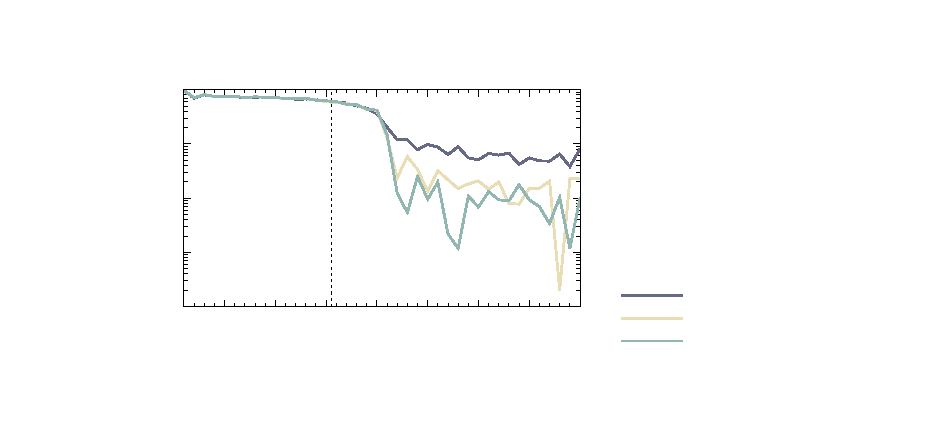
\includegraphics[width={432.00bp},height={188.60bp}]{../Plots/AllMaterials/Mu-1.5/plot}}%
    \gplfronttext
  \end{picture}%
\endgroup

